% Unofficial LaTex beamer theme for Seoul National University
%
% Copyright 2014 Lucy Park <ejpark04@snu.ac.kr>
% http://lucypark.kr
%
% This file may be distributed and/or modified under the GNU GPL 3.0 or above
% http://www.gnu.org/licenses/gpl-3.0.html
%

\documentclass[compress]{beamer}
\usepackage{beamerthemeshadow}
\usetheme{snubeam}

\begin{document}
\title{Unofficial LaTex beamer theme \\for Seoul National University}
\author{Lucy Park}
\institute{
    Data Mining Center\\
    College of Engineering\\
    Seoul National University}
\date{\today}

{
\usebackgroundtemplate{
\includegraphics[width=\paperwidth]{images/snu-shift}}
\begin{frame}[plain]
  \titlepage
\end{frame}
}


\begin{frame}\frametitle{Table of contents}
    \tableofcontents
\end{frame}


\section{서론}
\begin{frame}\frametitle{Hello world!}
    This is a unofficial beamer theme for Seoul National University.
    \footnote{http://snu.ac.kr}
\end{frame}


\section{본론}
\subsection{Lists}
\begin{frame}\frametitle{Unnumbered lists}
    \begin{itemize}
        \item Introduction to  \LaTeX
        \item Termpapers and presentations with \LaTeX
        \item Beamer class
    \end{itemize}
\end{frame}
\begin{frame}\frametitle{Lists with pause}
    \begin{itemize}
        \item Introduction to  \LaTeX \pause
        \item Termpapers and presentations with \LaTeX \pause
        \item Beamer class
    \end{itemize}
\end{frame}
\begin{frame}\frametitle{Numbered lists}
    \begin{enumerate}
        \item Introduction to  \LaTeX
        \item Termpapers and presentations with \LaTeX
        \item Beamer class
    \end{enumerate}
\end{frame}
\begin{frame}\frametitle{Numbered lists with pause}
    \begin{enumerate}
        \item Introduction to  \LaTeX \pause
        \item Termpapers and presentations with \LaTeX \pause
        \item Beamer class
    \end{enumerate}
\end{frame}

\subsection{Tables}
\begin{frame}\frametitle{Tables}
    \begin{tabular}{|c|c|c|}
        \hline
        \textbf{Date} & \textbf{Organizer} & \textbf{Title} \\ \hline
        2014-08-24 & Lucy & Create \LaTeX template \\ \hline
        2014-08-30 & PyCon & Korean NLP \\ \hline
    \end{tabular}
\end{frame}

\subsection{Blocks}
\begin{frame}\frametitle{Blocks}
    \begin{block}{title of the bloc}
        bloc text
    \end{block}
    \begin{exampleblock}{title of the bloc}
        bloc text
    \end{exampleblock}
    \begin{alertblock}{title of the bloc}
        bloc text
    \end{alertblock}
\end{frame}

\subsection{Layout}
\begin{frame}\frametitle{Splitting screens}
    \begin{columns}
        \begin{column}{5cm}
            \begin{itemize}
                \item Beamer
                \item Beamer Class
                \item Beamer Class Latex
            \end{itemize}
        \end{column}
        \begin{column}{5cm}
            \begin{tabular}{|c|c|}
                \hline
                \textbf{Organizer} & \textbf{Title} \\ \hline
                Lucy &  \LaTeX template \\ \hline
                PyCon & Korean NLP \\
                \hline
            \end{tabular}
        \end{column}
    \end{columns}
\end{frame}

\subsection{Pictures}
\begin{frame}\frametitle{Pictures in latex beamer class}
    \begin{figure}
        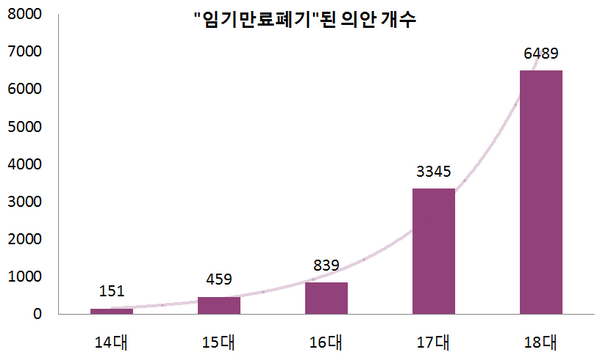
\includegraphics[scale=0.5]{images/graph.png}
        \caption{show an example picture}
    \end{figure}
\end{frame}
\begin{frame}[plain]
    \frametitle{Plain, or a way to get more space}
    \begin{figure}
        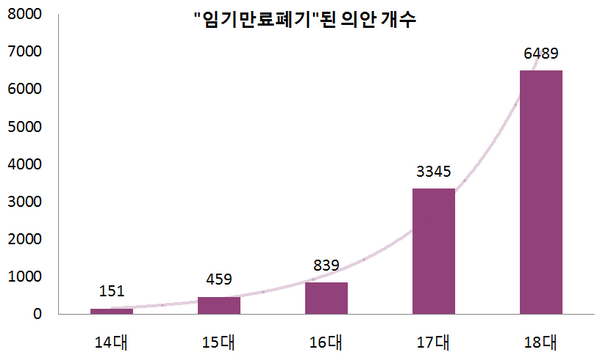
\includegraphics[scale=0.5]{images/graph.png}
        \caption{show an example picture}
    \end{figure}
\end{frame}


\section{결론}
\begin{frame}\frametitle{Send your suggestions}
    \vfill
    \begin{center}
        \begin{Huge}감사합니다.\end{Huge}\\
        \url{http://github.com/e9t/snubeam}
    \end{center}
    \vfill
\end{frame}

\begin{frame}[t, allowframebreaks]\frametitle{References}
    \nocite{*} % FIXME: this includes all references in ref.bib
    \bibliography{ref}
\end{frame}
\end{document}
